\chapter{Experiments and Evaluation}
\label{evaluation}
% DELETEME: The evaluation chapter is one of the most important chapters of your work. Here, you will prove usability/efficiency of your approach by presenting and interpreting your results. You should discuss your results and interpret them, if possible. Drawing conclusions on the results will be one important point that your estimators will refer to when grading your work.

This chapter serves as a presentation of the actors used in our experiments, and the output of the camera, after which is discussed if it has met the expectations and whether the approach was efficient in providing a solution for the CPO problem.

\section{Experiments}
In this thesis, two different experiments were conducted in order to evaluate the performance loss of cameras. What is more, with the help of heatmaps and using the metrics M1 and M2 we are able to define an optimal camera position. The experiments aim to check if problems from Chapter \ref{problem_analysis} are handled efficiently by the proposed strategy. In the next subsections, we inform about the laptop used for our simulations and explain into details each experiment. Afterwards, we discuss the results and the efficiency of our metrics.

\subsection{Technical specifications}
The following list contains technical specifications of the machine, which all experiments were simulated on:
\begin{itemize}
    \item \textbf{Processor} - Intel Core i7-10750H CPU 2.60GHz
    \item \textbf{RAM} - 16 GB DDR5
    \item \textbf{GPU} - NVIDIA GeForce RTX 3060 6 GB
    \item \textbf{SSD} - 1 TB
\end{itemize}

\newpage
\subsection{First experiment - change height and angle of camera}
The main objective of our first experiment is to evaluate the performance of cameras at different height, because we concluded from the found literature in Chapter \ref{problem_analysis} that there is little information about which height is optimal for traffic surveillance. We use heatmaps to present the maximal occlusion degree for each spawn point. Additionally, our metric M2 is applied in order to see what part from all cases were occlusions and choose these positions which have scored lower values. During the execution of simulations, we rely on a camera with the following configurations:
\begin{itemize}
    \item FoV (horizontal angle) = $80^{\circ}$
    \item Resolution = $1280\times720$ pixels or also known as 720p
\end{itemize}
The reason for our horizontal angle is that we wanted to cover as much as possible from our region of interest and an average traffic surveillance camera on the market has a horizontal field of view $70^{\circ} - 110^{\circ}$. In a real-world scenario, a wider field of view will cause a fisheye effect\footnote{When an image is distorted by stretching the picture around a rounded camera lens} to occur and has to be taken into account. However, in our experiments the conditions are ideal and we do not apply image distortion. We have 8 enumerated positions for the camera, which can be seen in Figure \ref{fig:positions_enumerated}, where we place it at a pre-defined height. On each of these spawn locations for our sensor, we define 6 levels for the height beginning at 5 meters and going up to 10 meters with a 1-meter step. This results in 48 simulations, where we set $0^{\circ}$ for the tilt angle at 5 meters, $-10^{\circ}$ at 6 meters and then reach up to $-30^{\circ}$ at 10 meters with a $-5^{\circ}$ step. In this way, we guarantee that the camera has approximately the same sight over the vehicles and the blind spot under the sensor does not increase. The region of interest, which comprises the four-road intersection, is limited by the red lines in Figure \ref{fig:positions_enumerated} and is used in each of the two experiments.

During each simulation, we generate a list with waypoints for the target vehicle that are 3 meters apart and one for the occluder, but with 1-meter distance between spawn points. We decided to use Seat Leon (see Fig. \ref{fig:seat_leon}) as a target and Jeep Wrangler Rubicon (see Fig. \ref{fig:jeep_wrangler}) as an occluder for our scenarios, because in an urban area people mainly utilise normal cars or SUVs for their transportation needs, and therefore it is more often the case that these two types of vehicles are captured by a camera. In our second experiment, we consider pairs of vehicles of different type in order to broaden the variety of measured occlusions.

\begin{figure} [h!]
    \centering
    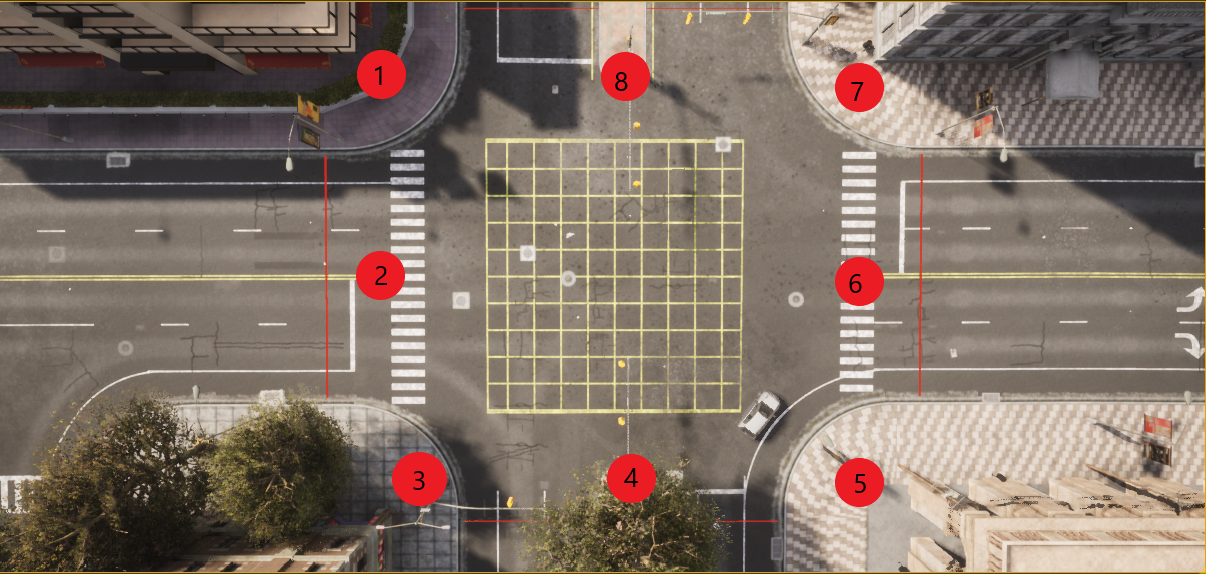
\includegraphics[width=0.90\textwidth]{images/positions_numerated.png}
    \caption[Enumerated camera positions]{This image shows the number of each camera's position examined in our simulations.}
    \label{fig:positions_enumerated}
\end{figure}

\newpage
\subsection{Second experiment - change threshold for target vehicle recognition}
In our second experiment our goal is to observe how strong the occlusion is when there are different types of vehicles. Here we use the same parameters for the camera, but this time it is placed only at 8 meters above the ground. The reason behind this decision is that we have mentioned in Section \ref{main_problems} that the minimum for an ideal height is exactly 8 meters. Furthermore, we guarantee same conditions for all sensor positions by setting their tilt angle at $-20^{\circ}$ in order to have an accurate comparison. For this scenario, we use three pairs of vehicles and execute a simulation for 6 camera positions, which comprises a total of 18 simulations, 6 of which are also part of the first experiment. Moreover, we decided to not consider positions 4 and 8 here, because their view is obstructed by the traffic lights and hanging signs on their poles, therefore their range of view is limited.

For this experiment we rely on the pairs:
\begin{itemize}
    \item Seat Leon and Jeep Wrangler Rubicon
    \item Ford Mustang and Mercedes Sprinter (see Figures \ref{fig:ford_mustang} and \ref{fig:mercedes_sprinter})
    \item Ambulance truck (see Fig. \ref{fig:ambulance}) and Mercedes Sprinter
\end{itemize}
Our idea is to reproduce three possible traffic scenarios, in which we have a normal car and SUV, a normal car and a large van, as well as two large-sized vehicles. In this way, we can ensure that a variety of vehicles' sizes are covered by this study. Important to mention is that the distance between target spawn points is again set to 3 meters. 

For the purpose of assessing optimal camera locations, we apply our M1 metric for a priori specified threshold. In the real world it is vital for a camera to miss as little as possible objects, which were hidden due to other large-sized vehicles. Therefore, we set an occlusion tolerance threshold, after which the target vehicle is no more detectable, to 50\%, 75\% and 90\%. By implementing this constraint, we can conclude from the score of our metric how many occlusions from all the detected ones could actually blind the camera. Finally, we choose these positions, which output the lowest values. Apart from the metric, heatmaps display the maximum occlusion degree for each target position, captured by the sensor.

%###################################################################################
%###################### Results             ########################################
%###################################################################################
\section{Results}\label{results}
In the heatmaps and tables below, we can inspect the results from both experiments. In order to maintain a well-arranged visualisation of the output, we are going to present only the heatmaps for 5 and 10-meter height and compare the impact of increasing elevation on the maximum occlusions. For our second experiment, we will visualise the results from cameras placed at 8 meters above the road in positions 1, 3 and 6. The other heatmaps are placed in the appendix 
\ref{appendix_heatmaps}, if one wants to analyse them.

\subsection{First experiment} \label{subsec:first_exp_heat}

\begin{figure}[!htb]
\minipage{0.5\textwidth}
  \includesvg[width=\linewidth]{images/position0/pos0_5m.svg}
  \caption{Pos.1 at 5 m height}\label{fig:pos1_5m}
\endminipage\hfill
\minipage{0.5\textwidth}
  \includesvg[width=\linewidth]{images/position0/pos0_10m.svg}
  \caption{Pos.1 at 10 m height}\label{fig:pos1_10m}
\endminipage\hfill
\end{figure}

\newpage
\begin{figure}[!ht]
\minipage{0.5\textwidth}
  \includesvg[width=\linewidth]{images/position1/pos1_5m.svg}
  \caption{Pos.2 at 5 m height}\label{fig:pos2_5m}
\endminipage\hfill
\minipage{0.5\textwidth}
  \includesvg[width=\linewidth]{images/position1/pos1_10m.svg}
  \caption{Pos.2 at 10 m height}\label{fig:pos2_10m}
\endminipage\hfill
\end{figure}

\begin{figure}[!ht]
\minipage{0.5\textwidth}
  \includesvg[width=\linewidth]{images/position2/pos2_5m.svg}
  \caption{Pos.3 at 5 m height}\label{fig:pos3_5m}
\endminipage\hfill
\minipage{0.5\textwidth}
  \includesvg[width=\linewidth]{images/position2/pos2_10m.svg}
  \caption{Pos.3 at 10 m height}\label{fig:pos3_10m}
\endminipage\hfill
\end{figure}

\begin{figure}[!ht]
\minipage{0.5\textwidth}
  \includesvg[width=\linewidth]{images/position3/pos3_5m.svg}
  \caption{Pos.4 at 5 m height}\label{fig:pos4_5m}
\endminipage\hfill
\minipage{0.5\textwidth}
  \includesvg[width=\linewidth]{images/position3/pos3_10m.svg}
  \caption{Pos.4 at 10 m height}\label{fig:pos4_10m}
\endminipage\hfill
\end{figure}

\newpage
\begin{figure}[!ht]
\minipage{0.5\textwidth}
  \includesvg[width=\linewidth]{images/position4/pos4_5m.svg}
  \caption{Pos.5 at 5 m height}\label{fig:pos5_5m}
\endminipage\hfill
\minipage{0.5\textwidth}
  \includesvg[width=\linewidth]{images/position4/pos4_10m.svg}
  \caption{Pos.5 at 10 m height}\label{fig:pos5_10m}
\endminipage\hfill
\end{figure}

\begin{figure}[!ht]
\minipage{0.5\textwidth}
  \includesvg[width=\linewidth]{images/position5/pos5_5m.svg}
  \caption{Pos.6 at 5 m height}\label{fig:pos6_5m}
\endminipage\hfill
\minipage{0.5\textwidth}
  \includesvg[width=\linewidth]{images/position5/pos5_10m.svg}
  \caption{Pos.6 at 10 m height}\label{fig:pos6_10m}
\endminipage\hfill
\end{figure}

\begin{figure}[!ht]
\minipage{0.5\textwidth}
  \includesvg[width=\linewidth]{images/position6/pos6_5m.svg}
  \caption{Pos.7 at 5 m height}\label{fig:pos7_5m}
\endminipage\hfill
\minipage{0.5\textwidth}
  \includesvg[width=\linewidth]{images/position6/pos6_10m.svg}
  \caption{Pos.7 at 10 m height}\label{fig:pos7_10m}
\endminipage\hfill
\end{figure}

\newpage
\begin{figure}[!htb]
\minipage{0.5\textwidth}
  \includesvg[width=\linewidth]{images/position7/pos7_5m.svg}
  \caption{Pos.8 at 5 m height}\label{fig:pos8_5m}
\endminipage\hfill
\minipage{0.5\textwidth}
  \includesvg[width=\linewidth]{images/position7/pos7_10m.svg}
  \caption{Pos.8 at 10 m height}\label{fig:pos8_10m}
\endminipage\hfill
\end{figure}

\begin{table}[!h]
\caption{This table presents the M2 score of each camera position at different height level \label{tab:height_experiment}}
\centering
    \begin{tabular}{ | c | c | c | c | c | c | c | c | c |}
    \hline
    Height & Pos.1 & Pos. 2 & Pos. 3 & Pos. 4 & Pos. 5 & Pos. 6 & Pos. 7 & Pos. 8 \\ \hline
    5 m & 0.50 & 0.49 & 0.70 & 0.52 & 0.54 & 0.55 & 0.74 & 0.68\\ \hline
    6 m & 0.49 & 0.48 & 0.66 & 0.45 & 0.53 & 0.53 & 0.73 & 0.63\\ \hline
    7 m & 0.47 & 0.48 & 0.65 & 0.49 & 0.51 & 0.52 & 0.71 & 0.64\\ \hline
    8 m & 0.48 & 0.47 & 0.63 & 0.48 & 0.51 & 0.50 & 0.68 & 0.61\\ \hline
    9 m & 0.48 & 0.46 & 0.61 & 0.44 & 0.50 & 0.49 & 0.63 & 0.58\\ \hline
    10 m & 0.46 & 0.44 & 0.57 & 0.33 & 0.47 & 0.46 & 0.61 & 0.55\\ \hline
    \end{tabular}
\end{table}

\newpage
\subsection{Second experiment}

\begin{figure}[!htb]
\minipage{0.5\textwidth}
  \includesvg[width=\linewidth]{images/position0/pos0_8m.svg}
  \caption{Pos.1 Seat and Jeep}\label{fig:pos1_8m}
\endminipage\hfill
\minipage{0.5\textwidth}
  \includesvg[width=\linewidth]{images/mustang_sprinter/sprinter_mustang_pos0.svg}
  \caption{Pos.1 Ford and Mercedes}\label{fig:pos1_ford_merc}
\endminipage\hfill
\end{figure}

\newpage
\begin{figure}[!htb]
\minipage{0.5\textwidth}
  \includesvg[width=\linewidth]{images/sprinter_ambulance/ambulance_sprinter_pos0.svg}
  \caption{Pos.1 Ambulance and Mercedes}\label{fig:pos1_amb_merc}
\endminipage\hfill
\minipage{0.5\textwidth}
  \includesvg[width=\linewidth]{images/position2/pos2_8m.svg}
  \caption{Pos.3 Seat and Jeep}\label{fig:pos3_8m}
\endminipage\hfill
\end{figure}

\begin{figure}[!htb]
\minipage{0.5\textwidth}
  \includesvg[width=\linewidth]{images/mustang_sprinter/sprinter_mustang_pos2.svg}
  \caption{Pos.3 Ford and Mercedes}\label{fig:pos3_ford_merc}
\endminipage\hfill
\minipage{0.5\textwidth}
  \includesvg[width=\linewidth]{images/sprinter_ambulance/ambulance_sprinter_pos2.svg}
  \caption{Pos.3 Ambulance and Mercedes}\label{fig:pos3_amb_merc}
\endminipage\hfill
\end{figure}

\begin{figure}[!htb]
\minipage{0.5\textwidth}
  \includesvg[width=\linewidth]{images/position5/pos5_8m.svg}
  \caption{Pos.6 Seat and Jeep}\label{fig:pos6_8m}
\endminipage\hfill
\minipage{0.5\textwidth}
  \includesvg[width=\linewidth]{images/mustang_sprinter/sprinter_mustang_pos5.svg}
  \caption{Pos.6 Ford and Mercedes}\label{fig:pos6_ford_merc}
\endminipage\hfill
\end{figure}

\newpage
\begin{figure}[!htb]
\minipage{0.5\textwidth}
    \includesvg[width=\linewidth]{images/sprinter_ambulance/ambulance_sprinter_pos5.svg}
  \caption{Pos.6 Ambulance and Mercedes}\label{fig:pos6_amb_merc}
\endminipage\hfill
\end{figure}

\begin{table}[!htb]
\caption{This table presents the M1 score at 8 m height for a specified threshold and vehicles Seat Leon and Jeep Wrangler Rubicon\label{tab:jeep_seat_threshold}}
\centering
    \begin{tabular}{ | c | c | c | c | c | c | c |}
    \hline
    Threshold & Pos. 1 & Pos. 2 & Pos. 3 & Pos. 5 & Pos. 6 & Pos. 7 \\ \hline
    50\% & 0.17 & 0.22 & 0.06 & 0.11 & 0.17 & 0.09\\ \hline
    75\% & 0.02 & 0.06 & 0.01 & 0.01 & 0.03 & 0.0\\ \hline
    90\% & 0.0 & 0.0 & 0.01 & 0.0 & 0.0 & 0.0\\ \hline
    \end{tabular}
\end{table}

\newpage
\begin{table}[!htb]
\caption{This table presents the M1 score at 8 m height for a specified threshold and vehicles Ford Mustang and Mercedes Sprinter\label{tab:ford_merc_threshold}}
\centering
    \begin{tabular}{ | c | c | c | c | c | c | c |}
    \hline
    Threshold & Pos. 1 & Pos. 2 & Pos. 3 & Pos. 5 & Pos. 6 & Pos. 7 \\ \hline
    50\% & 0.38 & 0.48 & 0.39 & 0.36 & 0.44 & 0.41\\ \hline
    75\% & 0.24 & 0.31 & 0.21 & 0.18 & 0.26 & 0.22\\ \hline
    90\% & 0.15 & 0.18 & 0.12 & 0.12 & 0.14 & 0.12\\ \hline
    \end{tabular}
\end{table}

\begin{table}[!htb]
\caption{This table presents the M1 score at 8 m height for a specified threshold and vehicles Ambulance Truck and Mercedes Sprinter\label{tab:amb_merc_threshold}}
\centering
    \begin{tabular}{ | c | c | c | c | c | c | c |}
    \hline
    Threshold & Pos. 1 & Pos. 2 & Pos. 3 & Pos. 5 & Pos. 6 & Pos. 7 \\ \hline
    50\% & 0.08 & 0.15 & 0.08 & 0.07 & 0.12 & 0.09\\ \hline
    75\% & 0.0 & 0.0 & 0.0 & 0.0 & 0.0 & 0.0\\ \hline
    90\% & 0.0 & 0.0 & 0.0 & 0.0 & 0.0 & 0.0\\ \hline
    \end{tabular}
\end{table}

%###################################################################################
%###################### Discussions         ########################################
%###################################################################################
\newpage
\section{Discussions}\label{discussions}
In this section we are going to analyse the above displayed heatmaps and tables in order to compare camera's performance in various situations and decide which positions brought the most optimal results. Furthermore, we discuss which height levels were beneficial to the efficiency of our visual sensor.

\subsection{Results of first experiment}
To start with, if we examine the heatmaps from Subsection \ref{subsec:first_exp_heat} and Table \ref{tab:height_experiment}, then we can assert that height is actually of utmost importance for the quantity of detected occlusions. For instance, in Figure \ref{fig:pos1_5m} and Figure \ref{fig:pos1_10m} it is noticeable that the difference of 5 meters significantly decreases the degree of occlusion for each target's spawn location. We are also able to see that our tilt angle is set correctly according to the height and ensures that the same spawn positions remain visible for the camera and new ones also appear at 10 meters. In Figure \ref{fig:pos1_8m} there are some occlusions over 80\%, which still does not achieve the goal we are looking for. 

Out of all positions, there are two offering a lower performance than the other ones - positions 4 and 8. The reason for this behaviour is that there are traffic lights and street signs hanging from the poles, which obstruct their view of the whole region of interest. Moreover, this setback also deprives them of detecting some locations on the road, which results in less evaluated situations, as can be asserted from heatmaps \ref{fig:pos4_5m} and \ref{fig:pos8_5m}. However, this outcome proves that our check for points out of the camera's field of view works properly and could also be applied to future experiments for a real-world scenarios.

For this study, it is of interest that fewer occlusions are detected from a certain position, therefore we used our metric M2 to evaluate which location is efficient for the task. In the table \ref{tab:height_experiment} it can be instantly seen that positions 1 and 2 have scored some of the lowest values at 5-meter height. However, if we take into account the M2 score of positions 4 and 8, they seem to outperform other camera locations, which is not correct information. As we mentioned previously, when a sensor is placed there its FoV is limited and sees half the recognisable spawn points. For this reason, their scores will be only valid, if approximately the same amount of target points are available on the image plane. Another important point to be made after examining the table is that with increase of height, the number of occlusion decreases, which is to be expected due to the fact that the sensor's view angle to the vehicles changes and can monitor them from an unhindered point of view in comparison to the lower heights. At 5, 6 and 7 meters our camera does not show a significant difference in the number of detected occlusions, whereas at a height over 8 meters the sensor tends to identify with 10-15\% fewer occlusions. With the output of our first experiment, we can consider the statement that an ideal height for a traffic camera starts at 8-meter (see \ref{main_problems}) height as correct.

Finally, after inspecting the heatmaps and the M2 score for each camera placement, positions 1, 2, 3 and 7 guarantee a better range of view compared to the others, because they have had a larger number of target spawn points in their sight during the experiment. With regard to the quantity of occlusion on the heatmaps for 10-meter height, position 3 seems to avoid them more efficiently, although its M2 score is the third highest in the table, where 57\% of all cases were occlusions. This metric seems to be inaccurate when comparing the score at the same height in different positions, because in some of them the camera detect more points around the target vehicle, which allows for more non-occlusion situations and thus the smaller score. In conclusion, we can say that higher placement is crucial, because there are almost no physical view obstructors. Additionally, an optimal range of view implies better perception of the environment, like it is guaranteed by positions 1, 2, 3 and 7.

\subsection{Results of second experiment}
During this experiment were involved different types of vehicles, which led to a better overview of how the occluder's size affects the number of occlusion occurrences. For example, when we compare heatmaps \ref{fig:pos1_8m} and \ref{fig:pos1_ford_merc}, it gets clear that a camera at the height of 8 meters has a more obstructed view when a Mercedes Sprinter stays in front of a Ford Mustang than in the case when a Jeep Wrangler Rubicon acts as occluder. This ensuing performance we explain by the fact that a Mercedes Sprinter is $2,5-3 m$ tall and for this reason a larger blind zone is formed behind it. Moreover, independent of camera's position this phenomenon occurs in each of the simulations at the height of 8 meters, therefore it is reasonable to place a camera on a higher level above the road, otherwise there will be decrease in the sensor's performance.

If we look at Figures \ref{fig:pos6_8m} and \ref{fig:pos6_amb_merc} we notice that there is only a slight difference in the detected occlusion degree, which is due to approximately the same size of the vehicles. What we find surprising in position 6 is that the Mercedes Sprinter has caused less occlusion on the ambulance truck in comparison to the Jeep Wrangler Rubicon, but in our opinion the larger size of the trucks is to blame for it. To provide further explanation, more pixels on the image plane represent the ambulance truck as opposed to the Seat Leon, therefore the occlusion degree by the first vehicle increases slower. Nevertheless, if we consider the results from the other heatmaps, it seems that problematic for the sensor are only cases where the occluder vehicle is taller than the target one.

Apart from the heatmaps, we also applied our M1 metric for this experiment in order to investigate what part of all detected occlusions are the ones that exceed a pre-defined threshold. To start with, from Table \ref{tab:jeep_seat_threshold} we realise that in positions 3 and 7 have been detected less than 10\% of occlusions, whose degrees were above 50\%. In a real-world situation, 50\% occlusion should not burden an object recognition algorithm, but still to have less severe occlusions monitored is our objective. Subsequently, in the third row the occlusion degrees above 90\% for each position are between 0 and 1\%, which is expected due to the near sizes of both Seat Leon and Jeep Wrangler Rubicon. What is more, it is a rare case that same-sized vehicles cause a full view obstruction to each other, when a camera is placed at least 8 meters above them.

However, if we have a look at Table \ref{tab:ford_merc_threshold}, the values change considerably, as there have been calculated more than 35\% occlusions whose degrees were above 50\%. According to the results, camera positioned at 8 meters is not reliable because it detects numerous occlusions, when we there are trucks or vans on the street which cover the normal cars. Out of all positions 3, 5 and 7 offer a promising performance even in such environmental conditions. On the contrary, positions 2 and 6 tend to suffer more efficiency loss than the other locations, which is due to their rather central position and field of view. As it is illustrated by the heatmaps \ref{fig:pos6_5m} and \ref{fig:pos2_5m}, the number of target spawn points that have been detectable from the camera is low.

Finally, in Table \ref{tab:amb_merc_threshold} we notice that little occlusion occurs between the large-sized vehicles when the threshold is 50\% while above 75\% no occlusion has been recorded, which is an optimal result in case of two big vehicles crossing the junction. Taking everything into consideration, positions 3, 5 and 7 have scored the lowest M2 values, which mean they perform well independent of the vehicles' sizes and types.

After having examined and analysed the results of both experiments in detail, we can advance the opinion that positions 3 and 7 outperform the other ones and offer a balance between number of detected spawn locations and perceived occlusion degree. Definitely, cameras on a higher level (min. 8 m) above the ground have an increased visibility over the road and decrease the blind zone caused by taller vehicles. 

\subsection{Efficiency of metrics} \label{subsec:efficiency_metrics}
As we have seen in the previous subsections, two metrics (M1 and M2) were essential for arriving at a decision about which position and which height contribute to an enhanced camera efficiency. Their role in our approach, as described in Section \ref{subsec:metrics}, was to distinguish which occlusions were greater than a pre-defined threshold and to calculate how many out of all examined situations delivered an occlusion. After we have inspected the results, it can be assumed that they fulfilled their task and aided us in determining areas where a camera performs promisingly. However, there were two drawbacks that arose:
\begin{enumerate}
    \item M2 is more appropriate, when one investigates the behaviour of the camera at a different height in the same position. For correct results, the tilt angle should be adjusted like in our experiments, then the camera can see an identical number of spawn points, because the FoV does not change. If, however, we want to compare positions 3 and 4, we will see in Table \ref{tab:height_experiment} that the second one outputs lower values, which could lead us to a wrong conclusion about the two positions. Therefore, heatmaps were also involved in the data visualisation, which implied that position 4 has observed 50\% fewer spawn locations and in this way the M2 score gets unreliable. For the purpose of avoiding this issue, it is advisable to extend the metric and compare as well the number of monitored spawn points when studying two positions. Thus, it is ensured that the value of the metric is not influenced by side aspects.
    \item M1 is responsible for evaluating what part of all situations that resulted in occlusion denotes a value which exceeds a threshold for object recognition. Overall, it was accurate and served its role, but does not bring valuable information, as it can be seen at the second two rows in tables \ref{tab:jeep_seat_threshold} and \ref{tab:amb_merc_threshold}, when vehicles of the same size are compared. In our case, cameras were placed at 8 meters above the vehicles, from where it is impossible to detect occlusions larger than 80-90\%. However, if we consider the scenario in Table \ref{tab:ford_merc_threshold} where the occluder is significantly taller than the target vehicle, M1 provides useful data, because more occlusions land in the sensor's range of view. Therefore, instead of applying the M1 metric for same-sized vehicles at the same height, it is reasonable to compare the change in performance at different height levels (at least 8 meters) and using a truck as occluder. In this way, worst-case scenarios can be examined, which is important for generating precise results for a real-world implementation. 
\end{enumerate}
